% Created 2020-10-25 So 23:03
% Intended LaTeX compiler: pdflatex
\documentclass[11pt]{scrartcl}
\usepackage[utf8]{inputenc}
\usepackage[T1]{fontenc}
\usepackage{graphicx}
\usepackage{grffile}
\usepackage{longtable}
\usepackage{wrapfig}
\usepackage{rotating}
\usepackage[normalem]{ulem}
\usepackage{amsmath}
\usepackage{textcomp}
\usepackage{amssymb}
\usepackage{capt-of}
\usepackage{MnSymbol}
\usepackage{mathtools}
\usepackage{setspace}
\usepackage{nicematrix}
\usepackage{listings}
\usepackage{pdfpages}
\usepackage[straightvoltages, european resistors, american inductors]{circuitikz}


\author{David Keller, Moritz Woltron, Matthias Fottner}
\date{}
\title{Protokoll Übung 1}




\definecolor{darkspringgreen}{rgb}{0.09, 0.45, 0.27}    % Farbe für die Kommentare bei Listings
\lstset{
  language= Matlab,                     % Setzt die Sprache
  basicstyle=\scriptsize\ttfamily,     % Setzt den Standardstil
  % keywordstyle=\color{red}\bfseries,    % Setzt den Stil für Schlüsselwörter
  identifierstyle=\color{blue},        % Identifier bekommen keine gesonderte formatierung
  commentstyle=\color{darkspringgreen},        % Stil für Kommentare
  stringstyle=\ttfamily,             % Stil für Strings (gekennzeichnet mit "String")
  breaklines=true,             % Zeilen werden umgebrochen
  numbers=left,                 % Zeilennummern links
  numberstyle=\tiny,             % Stil für die Seitennummern
  frame=single,                 % Rahmen
  % backgroundcolor=\color{myGrey},     % Hintergrundfarbe
  % caption={Java-Code},             % Caption
  tabsize=2                % Größe der Tabulatoren
}




\begin{document}

\maketitle
\newcommand{\unit}[1]{\,\text{#1}}
\section{Schaltplan mit allen Strömen und Spannungen}
\begin{circuitikz}[scale=1.2]
        \draw (0,0) node(n0){};
        \draw (0,0) to[isource=$I_{S1}$, o-o] (0,4) node[label=left:$K_2$](n2){};
        \draw (n2) to[R=$R_1$, i=$I_{R1}$, v<=$U_{R1}$] ++ (0,4) to[short] ++ (4,0) node[label=above:$K_1$](n1){};
        \draw (n1) to[vsource=$U_{S2}$, i>=$I_{S2}^{?}$,  o-o] ++ (0, -4) node[label=north east:$K_3$](n3){};
        \draw (n2) to[R=$R_2$, i=$I_{R2}$, v=$U_{R2}$] (n3);
        \draw (n3) to[R=$R_5$, i=$I_{R5}$, v=$U_{R5}$, o-o] ++ (4,0) node[label=right:$K_4$](n4){};
        \draw (n1) to[short] ++ (4,0) to[cvsource=$U_{S3}$, i>=$I_{S3}^{?}$] (n4);
        \draw (n3) to[short] ++ (0,-1.5) node(n30){};
        \draw (n30) to[R=$R_3$, i=$I_{R3}$, v=$U_{R3}$] (4,0);
        \draw (n30) to[short] ++ (2.5,0) to[R=$R_4$, i=$I_{R4}$, v=$U_{R4}$] (6.5,0);
        \draw (6.5,0) to[short] (0,0);
        \draw (0,0) node[rground]{};

        % node voltages
        \draw[european voltages, color=green!50!black] (-0.8,8) to[open, v=$U_{n1}$] (-0.8,0);
        \draw[european voltages, color=green!50!black] (0.2 ,4) to[open, v^=$U_{n2}$] (0.2 ,0);
        \draw[european voltages, color=green!50!black] (n4) to[open, v^=$U_{n4}$] (7,0);
        \draw[european voltages, color=green!50!black] (n3) to[open, v=$U_{n3}$] (2,0);
\end{circuitikz}

\newpage
\section{Kirchhoff'schen Knotengleichungen}

\begin{doublespace}
K1: \(\displaystyle \quad I_{R1} + I_{S2}^? + I_{S3}^? = 0\) \\
K2: \(\displaystyle \quad I_{R2} - I_{S1} - I_{R1} = 0\)\\
K1: \(\displaystyle \quad I_{R5} + I_{R3} + I_{R4} - I_{R2} - I_{S2}^? = 0\) \\
K1: \(\displaystyle \quad -I_{R5} - I_{S3}^? = 0\)
\end{doublespace}

\subsection{Ohm'sches Gesetz}
\begin{spacing}{2.5}
K1: \(\displaystyle \quad \frac{U_{R1}}{R_1} + I_{S2}^? + I_{S3}^? = 0\) \\
K2: \(\displaystyle \quad \frac{U_{R2}}{R_2} - \frac{U_{R1}}{R_1} = I_{S1}\) \\
K3: \(\displaystyle \quad \frac{U_{R5}}{R_5} + \frac{U_{R3}}{R_3} + \frac{U_{R4}}{R_4} - \frac{U_{R2}}{R_2} - I_{S2}^? = 0\) \\
K4: \(\displaystyle \quad - \frac{U_{R5}}{R_5} - I_{S3}^? = 0\)
\end{spacing}

\subsection{Knotenspannungen}\label{sec:knotenspannungen}
\begin{doublespace}
\(\displaystyle U_{R3} = U_{R4} = U_{n3}\) \\
\(\displaystyle U_{R2} = U_{n2}- U_{n3}\) \\
\(\displaystyle U_{R1} = U_{n1}- U_{n2}\) \\
\(\displaystyle U_{R5} = U_{n3}- U_{n4}\)
\end{doublespace}

\subsection{Knotengleichungen mit Knotenspannungen}
\begin{spacing}{2.5}
  K1: \(\displaystyle \quad \frac{U_{n1} - U_{n2}}{R_1} + I_{S2}^? + I_{S3}^? = 0\) \\
  K2: \(\displaystyle \quad \frac{U_{n2} - U_{n3}}{R_2} - \frac{U_{n1} - U_{n2}}{R_1} = I_{S1}\) \\
  K3: \(\displaystyle \quad \frac{U_{n3} - U_{n4}}{R_5} + \frac{U_{n3}}{R_3} + \frac{U_{n3}}{R_4} - \frac{U_{n2} - U_{n3}}{R_2} - I_{S2}^?= 0\) \\
  K4: \(\displaystyle \quad - \frac{U_{n3} - U_{n4}}{R_5} - I_{S3}^? = 0\)
\end{spacing}

\subsection{zusätzliche Bedingungen}
\begin{itemize}
\item 6 Unbekannte: $U_{n1}, U_{n2}, U_{n3}, U_{n4}, I_{S2}^?, I_{S3}^?$
\item nur 4 Gleichungen: unbestimmtes Gleichungssystem
\item 2 weitere Gleichungen
\end{itemize}
\begin{align}
  U_{S2} &= U_{n1} - U_{n3} \\
  U_{S3} &= U_{n1} - U_{n4} = \alpha \cdot I_{R3} = \alpha \cdot \frac{U_{R3}}{R_3} = \alpha \cdot \frac{U_{n3}}{R_3} \nonumber \\
  \Longrightarrow 0 &= U_{n1} - U_{n4} - \alpha \cdot \frac{U_{n3}}{R_3}
\end{align}


\section{Gleichungssystem in Matrixform}
Definition Leitwerte: \(\displaystyle \quad G_n := \frac{1}{R_n}\)


\begin{equation*}
  \renewcommand{\arraystretch}{2}
    \underbrace{\left[\begin{NiceArray}{c:c:c:c:c:c}
    G_1 & -G_1 & 0 & 0 & 1 & 1 \\
    \hdottedline
    -G_1 & G_1 - G_2 & -G_2 & 0 & 0 & 0 \\
    \hdottedline
    0 & -G_2 & G_2 + G_3 + G_4 + G_5 & -G_5 & -1 & 0 \\
    \hdottedline
    0 & 0 & -G_5 & G_5 & 0 & -1 \\
    \hdottedline
    1 & 0 & -1 & 0 & 0 & 0 \\
    \hdottedline
    1 & 0 & -\alpha \cdot G_3 & -1 & 0 & 0
  \end{NiceArray}\right]}_{\text{A}} \ \cdot \
\underbrace{\left\{ \begin{NiceArray}{c}
    U_{n1} \\
    \hdottedline
    U_{n2} \\
    \hdottedline
    U_{n3} \\
    \hdottedline
    U_{n4} \\
    \hdottedline
    I_{S2}^? \\
    \hdottedline
    I_{S3}^?
  \end{NiceArray}\right\}}_{\text{x}} \ = \
\underbrace{\left\{ \begin{NiceArray}{c}
    0 \\
    \hdottedline
    I_{S1} \\
    \hdottedline
    0 \\
    \hdottedline
    0 \\
    \hdottedline
    U_{S2} \\
    \hdottedline
    0
  \end{NiceArray}
\right\}}_{\text{b}}
\end{equation*} \\

Nach x auflösen: \(\displaystyle \quad x = A^{-1} b \) \\

Mithilfe von Matlab erhält man:
\begin{equation*}
  \renewcommand{\arraystretch}{1.25}
  x = \left\{\begin{array}{c}
      U_{n1} \\
      U_{n2} \\
      U_{n3} \\
      U_{n4} \\
      I_{S2}^? \\
      I_{S3}^? \end{array}\right\} =
  \left\{ \begin{array}{c}
            5,2143 \unit{V}\\
    3,5476 \unit{V}\\
    1,7143 \unit{V}\\
    3,5000 \unit{V}\\
    -1,1310 \unit{A}\\
    0,2976 \unit{A} \end{array}\right\}
\end{equation*}

Mit diesen Werten und mithilfe der Knotenspannungsgleichungen aus \ref{sec:knotenspannungen} lassen sich die
Spannungen $U_{R1} ...  U_{R5}$ und die Ströme $I_{R1} ...  I_{R5}$ ermitteln:

\begin{equation*}
  \renewcommand{\arraystretch}{1.25}
  U = \left\{ \begin{array}{c}
                U_{R1} \\
                U_{R2} \\
                U_{R3} \\
                U_{R4} \\
                U_{R5} \\
                \end{array}
  \right\} =
  \left\{ \begin{array}{c}
                U_{n1} - U_{n2}\\
                U_{n2} - U_{n3} \\
                U_{n3} \\
                U_{n3} \\
                U_{n3} - U_{n4}
          \end{array}\right\} =
        \left\{ \begin{array}{c}
                  1,6667 \unit{V} \\
                  1,8333 \unit{V} \\
                  1,7143 \unit{V} \\
                  1,7143 \unit{V} \\
                  -1.7857 \unit{V}
                \end{array}\right\}
            \end{equation*}

            \begin{equation*}
              \renewcommand{\arraystretch}{1.25}
              I = \left\{ \begin{array}{c}
                            I_{R1} \\
                            I_{R2} \\
                            I_{R3} \\
                            I_{R4} \\
                            I_{R5}
                          \end{array}\right\} =
                        \left\{ \begin{array}{c}
                                  U_{R1} / R_1 \\
                                  U_{R2} / R_2 \\
                                  U_{R3} / R_3 \\
                                  U_{R4} / R_4 \\
                                  U_{R5} / R_5
                                \end{array}\right\} =
                              \left\{ \begin{array}{c}
                                        0.8333 \unit{A} \\
                                        1.8333 \unit{A} \\
                                        0.4286 \unit{A} \\
                                        0.5714 \unit{A} \\
                                        -0.2976 \unit{A}
                                      \end{array}\right\}
                                  \end{equation*}

                                  Die Quellspannung der stromgesteuerten Quelle $U_{S3}$ erhält man aus der Lösung der Knotenspannungen:
                                  \begin{equation*}
                                    U_{S3} = U_{n1} - U_{n4} = 1,7143 \unit{V}
                                  \end{equation*}

\section{Leistungsbilanz}
Für das Aufstellen der Leistungsbilanz ist wichtig, welche Vorzeichen die Spannungen und Ströme am jeweiligen Bauteil haben.
Zeigen Spannungs- und Stromzählpfeil in dieselbe Richtung, und sind auch die Vorzeichen gleich, so geht die Leistung an
diesem Bauteil positiv in die Bilanz ein.
Zeigen die Pfeile in die gleiche Richtung, aber die Vorzeichen sind unterschiedlich, so handelt es sich um eine negative Leistungsbilanz.
Bei unterschiedlicher Zählpfeilrichtung entspricht ein unterschiedliches Vorzeichen einer positiven Leistung, ansonsten einer negativen.
Alle Leistungsanteile im Netzwerk müssen entsprechend der Energieerhaltung 0 ergeben. \\
Man erkennt, dass alle Leistungsanteile an den Widerständen positiv zu bewerten sind.
Außerdem muss der Leistungsanteil der stromgesteuerten Spannungsquelle $S3$ positiv gewertet werden, da sowohl
Spannung als auch Strom positiv ist und die Zählpfeile die gleiche Richtung haben.
Man erhält für alle positiven Leistungen $P_p$:
\begin{align*}
  P_p &= U_{R1} \cdot I_{R1} +
        U_{R2} \cdot I_{R2} +
        U_{R3} \cdot I_{R3} +
        U_{R4} \cdot I_{R4} +
        U_{R5} \cdot I_{R5} +
        U_{S3} \cdot I_{S3}^? \\
      &= 7,5060 \unit{W}
      \end{align*}

und für alle negativen Leistungen an den Quellen $S1$ und $S2$:
\begin{align*}
  P_n &= -(I_{S1} \cdot U_{n2}) + U_{S2} \cdot I_{S2}^? \\
      &= -7,5060 \unit{W}
\end{align*}

Die Summe aller Leistungen ergibt so $P_p + P_n = 0 \unit{W}$.


\section{Simulation}
\begin{center}
  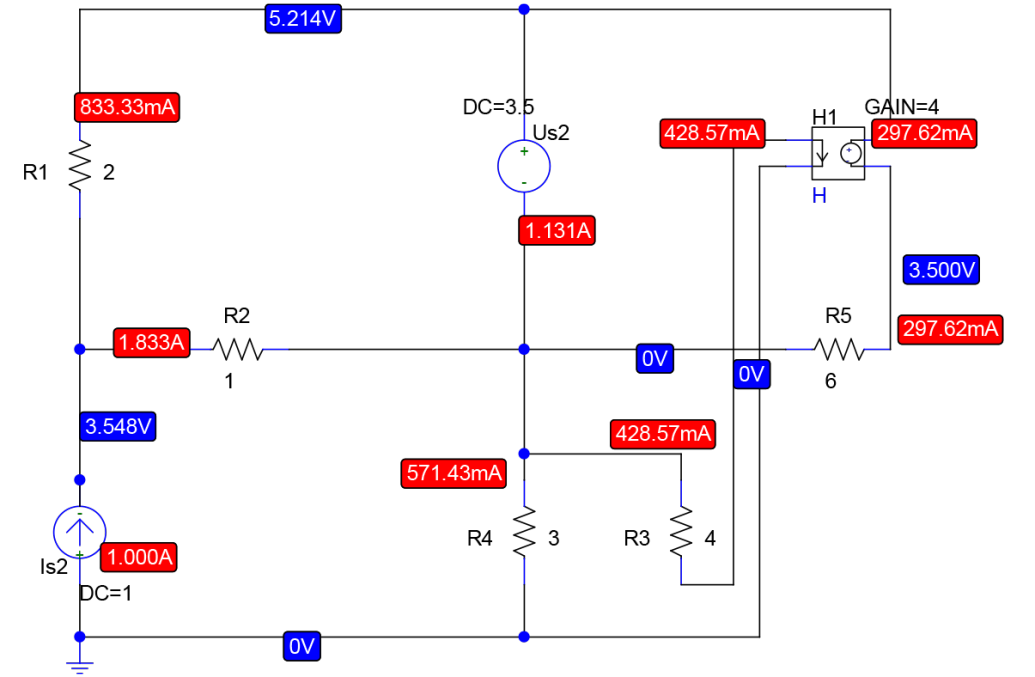
\includegraphics[width=.8\linewidth]{./Assets/PSpice_Schaltplan}
  \captionof{figure}{PSpice-Simulation des Netzwerks}
  \label{fig:A1}
\end{center}

\newpage
\section{Matlab-Skript}

\lstinputlisting[language=Matlab]{./Assets/Matlab_Ue01.m}

\end{document}
